\chapter{Makefile Examples}

\label{chap:examples}
This chapter includes examples of Makefiles included in the practical
data. We assume that you have unzipped the practical data into a
directory somewhere in your local environment. Once you have done
that, you should set an environment variable called
\texttt{MAKEPIPELINES} to refer to this directory. In the command below we assume you have placed it in your home directory:
\bashcmd{export MAKEPIPELINES=\textasciitilde{}/makepipelines}

The examples included below will reference this environment variable as necessary to find the correct files.

\newgeometry{scale=0.85, centering}
\definecolor{lemon}{HTML}{F5ECCE}

\lstset{language=make,backgroundcolor=\color{lemon},showstringspaces=false,
	gobble=8,
	basicstyle=\small\ttfamily,
	breaklines=true,
	escapeinside={\%*}{*}}


\chapter{Running FreeSurfer}
\def\sectionautorefname{Running Freesurfer}
\label{chap:freesurfer}

This is an example of how to use a makefile to execute FreeSurfer's longitudinal pipeline. Note that FreeSurfer itself is a large pipeline built using \texttt{make}. However, we do not need to know that if we treat the program \texttt{recon-all} as a single executable and show how to use \maken{} to call it. Here, the Makefile functions more as a way to permit parallel execution of \texttt{recon-all} rather than a way to track dependencies. 

The code for this example is in \texttt{oasis-longitudinal-example-small/freesurfer/Makefile}.

\setcounter{codehighlight}{0} % RESET THIS BEFORE EVERY LST LISTING
\begin{lstlisting}
	PROJHOME=$$MAKEPIPELINES/oasis-longitudinal-sample-small
	%*\lnote*SUBJECTS_DIR=$(PROJHOME)/freesurfer

	QA_TOOLS=/usr/local/freesurfer/QAtools_v1.1
	FREESURFER_SETUP = /usr/local/freesurfer/stable5_3/SetUpFreeSurfer.sh
	RECON_ALL = /usr/local/freesurfer/stable5_3/bin/recon-all $(RECON_FLAGS)	
	%*\lnote*RECON_FLAGS = -use-mritotal -nuintensitycor-3T -qcache -all  -notal-check

	%*\lnote*SHELL=/bin/bash
\end{lstlisting}

\lnum{1}FreeSurfer normally likes to work with all subjects in a single directory. We set the \maken{} variable \texttt{PROJHOME} for convenience, and the \texttt{SUBJECTS_DIR} because it is required by FreeSurfer. \\
\indent\lnum{2}Because we have multiple versions of FreeSurfer installed, and because it is possible to run FreeSurfer with different flags, we set several variables that describe what version of FreeSurfer and what options we are using in the Makefile. Note that the definition for \texttt{RECON_ALL} refers to \texttt{RECON_FLAGS} seemingly before it is set. Recall that \maken{} dereferences variables when it uses them, so the order that these variables are set does not matter. This is not like \texttt{bash}!\\
\indent\lnum{3}By default, \maken{} uses \texttt{/bin/sh} to interpret recipes. Sometimes this can cause confusion, because \texttt{sh} has only a subset of the functionality of \texttt{bash}. We can avoid such confusion by setting the \maken{} variable \texttt{SHELL} explicitly.


\begin{lstlisting}
	%*\lnote*SUBJECTS=$(notdir $(wildcard $(PROJHOME)/subjects/*))	
\end{lstlisting}

\lnum{4}We need to obtain a list of subject identifiers to process. Here, we form this list by using a wildcard to obtain all the subject directories in \texttt{PROJHOME} and then stripping away all the directory prefixes using the \texttt{notdir} call.


\begin{lstlisting}
	SESSION=1
	%*\lnote*inputdirs=$(SUBJECTS:%=%.t$(SESSION))

	%*\lnote*.PHONY: qa setup freesurfer

	%*\lnote*setup: $(inputdirs)

	%*\lnote*%.t$(SESSION):  $(PROJHOME)/subjects/%/visit$(SESSION)/mpr-1.nifti.nii.gz
            mkdir -p $@/mri/orig; \
        	cp $^ $@/mri/orig; \
        	cd $@/mri/orig; \
        	mri_convert mpr-1.nifti.nii.gz 001.mgz
\end{lstlisting}

\lnum{5}This Makefile is intended to handle a longitudinal acquisition. Normally, one indicates the timepoint (here, the \texttt{SESSION} variable indicates the timepoint) by appending some suffix to the subject identifier. Here, we append the suffix \texttt{.t1} to each subject identifier to indicate that we are processing the first session. To run the makefile on the second timepoint, one could either edit it, or set this variable when calling \maken{} as follows:
\bashcmd{make SESSION=2}

\indent\lnum{6}We define three targets that do not correspond to files, so these are denoted as phony targets.\\
\indent\lnum{7}The phony target \texttt{setup} depends upon the input directories we defined in \lnum{6}.\\
\indent\lnum{8}This recipe creates the input directories by transforming the first MPRAGE image from the subject directory into mgz format. More complicated recipes may include conditionally choosing one of multiple MPRAGE images, using two images if available, and so forth. 


\begin{lstlisting}
	freesurfer: $(inputdirs:%=%/mri/aparc+aseg.mgz)

	%*\lnote*%.t$(SESSION)/mri/aparc+aseg.mgz: $(PROJHOME)/subjects/%/visit$(SESSION)/mpr-1.nifti.nii.gz
        	rm -rf `dirname $@`/IsRunning.*
	        source $(FREESURFER_SETUP) ;\
        	export SUBJECTS_DIR=$(SUBJECTS_DIR) ;\
        	$(RECON_ALL) -subjid $*.t$(SESSION) -all
\end{lstlisting}

\lnum{9} FreeSurfer creates many output files when it runs. Here, we select one of the critical files that should exist upon successful completion, \texttt{mri/aparc+aseg.mgz} to be the target of this rule. It depends upon the directory having been created so that we can call \texttt{recon-all} by specifying the subject directory. You might think that it would be wise to specify multiple FreeSurfer output files as targets. In this case, if the multiple targets are specified using a pattern rule, the recipe would be executed only once to create the targets. However, if we did not use a pattern rule, the recipe could be executed once per target. This is clearly not the intended behavior. To avoid confusion, we usually pick a single late-stage output file to be the target.


\begin{lstlisting}
	%*\lnote*qa: $(inputdirs:%=QA/%)

	%*\lnote*QA/%: %
        	source $(FREESURFER_SETUP) ;\
        	$(QA_TOOLS)/recon_checker -s $*
\end{lstlisting}

\lnum{10}We can create a number of quality assurance (QA) images from the FreeSurfer directories using the \texttt{recon_checker} program. The \texttt{qa} target depends upon directories within the \texttt{QA} subdirectory. These are created by \texttt{recon_checker} in \lnum{12}.


\begin{lstlisting}
	%*\lnote*Makefile.longitudinal:
		$(PROJHOME)/bin/genctlongitudinalmakefile > $@
\end{lstlisting}

\lnum{11}After all the cross-sectional runs have been completed, we can run the longitudinal pipeline. The first step in this pipeline is to create an unbiased template from all timepoints for each subject. The second step is to longitudinally process each timepoint with respect to the template.

Here, we have a bit of a problem specifying these commands to \maken{} because each subject may have a different number of timepoints and subjects may be missing a timepoint that is not the first or last. The syntax of the \texttt{recon-all} command to create an unbiased template does not lend itself well to using wildcards to resolve these issues:
\bashcmd{recon-all -base <templateid> -tp <tp1id> -tp <tp2id> ... -all}

We solve these problems by writing a shell script that generates a correct Makefile (\texttt{Makefile.longitudinal}). This is an example of taking a ``brute force'' approach rather than trying to use pattern rules or something more sophisticated. It gets the job done.

The new makefile defines a target \texttt{longitudinal}, and can be called as follows, adding additional flags for parallelism.
\bashcmd{make -f Makefile.longitudinal longitudinal}

\section{Testsubject Main Makefile}
\label{example:testsubjectmakefile}

This is an example of a subject-specific makefile that includes
pipelines (written using \maken{}) that have been developed by several people to process different types of
subject-level MRI data. Because there is only one subject in
this example, this subject specific makefile is not a symbolic link,
as it is in the \texttt{oasis-longitudinal-sample-small} directory. 

The code for this example is in \texttt{\$MAKEPIPELINES/testsubject/test001/Makefile}. 

\setcounter{codehighlight}{0} % RESET THIS BEFORE EVERY LST LISTING
\begin{lstlisting}
	%*\lnote*.PHONY = etiv fast flex robex freesurferskullstrip 

	%*\lnote*FSL_DIR=/usr/share/fsl/5.0 

	STD_BRAIN=$(FSL_DIR)/data/standard/MNI152_T1_2mm.nii.gz 

	ifeq "$(origin MAKEPIPELINES)" "undefined"
	MAKEPIPELINES=/project_space/makepipelines 
	endif 

	%*\lnote*t1subj := $(shell pwd) 
	subject := $(notdir $(t1subj)) 

	PROJECT_HOME=$(MAKEPIPELINES)/testsubject/

	%*\lnote*include $(PROJECT_HOME)/lib/makefiles/help_system.mk 
	include $(PROJECT_HOME)/lib/makefiles/resting.mk 
	include $(PROJECT_HOME)/lib/makefiles/xfm.mk 
	include $(PROJECT_HOME)/lib/makefiles/fcconnectivity.mk 
	include $(PROJECT_HOME)/lib/makefiles/QA.mk 
	include $(PROJECT_HOME)/lib/makefiles/methodsgenerator.mk

	%*\lnote*export OMP_NUM_THREADS=1 

	SHELL=/bin/bash 

	%*\lnote*FLEXPATH=$(PROJECT_HOME)/bin/wmprogram/sb/cross_platform/scripts

\end{lstlisting}

\lnum{1} We begin by specifying our phony targets. These will be
defined later. 
\lnum{2} This line that sets \texttt{FSL_DIR} will be commented out in
your makefile, but you should find out where your version of FSL is
installed and make sure that it is correct. If we do not specify the
version of the programs that we run in a makefile, \maken{} will use
the individual's \texttt{PATH} variable to find them. Because
different people may have different \texttt{PATH} variables, this will
result in unpredictable results (the opposite of reproducibility!)
Recall that \maken{} inherits variables from your environment, and you
can override them by setting them.

\lnum{3} It is useful to have a variable to refer to the
subject. Here, we simply obtain the subject from the last part of the
directory name. This won't work for more complicated linking
structures as described in \nameref{sec:practicum2}. 

\lnum{4} We include lots of other makefiles that we need. This keeps
this makefile short and readable. 

\lnum{5} Certain programs do their own parallelization on computers
with multiple processing elements (cores). To turn this off, we
override the environment variable \texttt{OMP_NUM_THREADS}. This
allows us to use the \texttt{-j} flag to \maken{} to parallelize
execution of the entire makefile.

\lnum{6} FLEX is a program for white matter hyperintensity
quantification that we use for this project. This variable simply
specifies its location. If you do not have it installed you just won't
be able to run that part of the processing. It is not mandatory. 

\begin{lstlisting}
	 %*\lnote*FLAIR = $(shell if [ -f 00_NOFLAIR ] ; then echo false; else echo true; fi)

	 HAVET1 = $(shell if [ -f 00_NOT1 ] ; then echo false; else echo true; fi)

	 %*\lnote*ifeq ($(HAVET1),true)
	 %*\lnote*all: $(call print-help,all,Do skull stripping, etiv, HC volume calculation) T1_skstrip.nii.gz first etiv
	 else
	 all:  $(call print-help,all,Do skull stripping, etiv, HC volume calculation)
		@echo "Subject is missing T1 - nothing to do here."
	 endif
\end{lstlisting}

\lnum{7} In large and complicated studies, a certain type of image may
be missing, but this does not stop us from processing all the data
that we have. Here, we test for a FLAIR acquisition by looking for a
marker file in the directory called \texttt{00_NOFLAIR} (and similarly
for the T1). 

\lnum{8} Here we modify the target \texttt{all} depending on whether
or not the subject has a T1 image. We also use the help system
described in \nameref{sec:practicum4} to document what this target
does. 


\begin{lstlisting}
	T1_skstrip.nii.gz: T1.nii.gz 
		bet $< $@ -B

	robex: $(call print-help,robex,Alternate skull stripping with ROBEX) T1.nii.gz 
		$(PROJECT_HOME)/bin/ROBEX/runROBEX.sh T1.nii.gz T1_skstrip.nii.gz

	freesurferskstrip: $(call print-help,freesurferskullstrip, Alternate skull stripping with FreeSurfer) $(PROJECT_HOME)/freesurfer/$(subject)/mri/brain.mgz
		subj=$(subject) ;\
		mri_vol2vol --mov $(PROJECT_HOME)/freesurfer/$${subj}/mri/brain.mgz \
		--targ $(PROJECT_HOME)/freesurfer/$${subj}/mri/rawavg.mgz \
		--regheader --o brain-in-rawavg.mgz ;\
		mri_convert brain-in-rawavg.mgz brain-in-rawavg.nii.gz ;\
		fslreorient2std brain-in-rawavg.nii.gz T1_skstrip.nii.gz ;\
\end{lstlisting}

We have rules in this makefile for three methods of skull
stripping. The default is simply to call \texttt{bet} with the bias
correction option (which worked well on the data for the study this
makefile was modeled after). However, when this method did not work
well, we tried alternative methods using ROBEX and FreeSurfer. Note
that because the targets \texttt{robex} and \texttt{freesurferskstrip}
are phony, they can be created at any time and will always overwrite
\texttt{T1_skstrip.nii.gz}. 


\begin{lstlisting}
	etiv: $(call print-help, etiv, Estimation of ICV using enigma protocol) eTIV.csv

	brain_to_std.mat brain_to_std.nii.gz: T1_skstrip.nii.gz 
		flirt -in $< -ref $(STD_BRAIN) -omat $@ -out brain_to_std.nii.gz

	eTIV.csv: brain_to_std.mat
		%*\lnote*etiv=`$(PROJECT_HOME)/bin/mat2det brain_to_std.mat \
		| awk '{print $$2 }'` ;\
		echo  $(subject)","$$etiv > $@
\end{lstlisting}

We estimate intracranial volume (ICV) using the ENIGMA protocol (as described in
\nameref{sec:practicum3}). This approach calculates the inverse 
determinant of the linear transformation of the T1 image to standard
space. This is a scaling factor that we can multiply the volume of the
standard space brain by to obtain an estimated ICV volume. 

\lnum{9} Note that when calling the \texttt{mat2det} script and
echoing the results to a file, we need two dollar signs (\texttt{\$\$})
for every one that we intend to pass to the shell.  



\begin{lstlisting}
	 first: first_all_fast_firstseg.nii.gz T1.nii.gz hippo.csv

	 first_all_fast_firstseg.nii.gz : T1.nii.gz
		$(PROJECT_HOME)/bin/run_first_all_edit -s "L_Hipp,R_Hipp"  -d -i T1.nii.gz -o first

	 hippo.csv: first_all_fast_firstseg.nii.gz 
		rh=`fslstats $< -u 54 -l 52 -V|awk `{print $$2}'' ;\
		lh=`fslstats $< -u 18 -l 16 -V|awk `{print $$2}'' ;\
		echo $$lh $$rh > hippo.csv
\end{lstlisting}

We run FSL FIRST to calculate hippocampal volumes. We put these into a
comma separated value file to make it easy to remember how to extract
these numbers from the \texttt{first_all_fast_firstseg.nii.gz} and
check them (or include them in a QA report) although there is no
reason you could not write a separate program to gather them all.


\begin{lstlisting}
	 ifeq ($(FLAIR),true)
	 flex: $(call print-help,flex, Run flex for white matter hyperintensity quantification) flair.nii.gz flair_skstrip.hdr flair_skstrip_flwmt_lesions.hdr wmhstats.csv

	 flair_restore.nii.gz: flair.nii.gz
		fast -B -o flair -t 2 $<

	 flair_skstrip.nii.gz: flair_restore.nii.gz
		bet $< $@ -R

	 flair_skstrip.hdr: flair_skstrip.nii.gz 
		fslchfiletype ANALYZE $< $@

	 flair_skstrip_flwmt_lesions.hdr: flair_skstrip.hdr
		@echo "Flex processing " $< 
		$(FLEXPATH)/sb_flex -fl $< 

	 flair_skstrip_renamed.nii.gz: flair_skstrip.nii.gz
		cp $< $@

	 flair_wmh_mask.nii.gz: flair_skstrip_flwmt_lesions.hdr
		fslmaths $< -uthr 1 $@

	 else
	 flex:
		@echo No FLAIR, nothing to do
	 endif

	 wmhstats.csv: flair_skstrip_flwmt_lesions.hdr flair_skstrip_renamed.nii.gz
		@echo Writing wmhstats.csv 
		tot=`fslstats  flair_skstrip_renamed.nii.gz -V | awk `{print $$2}''; \
		wmh=`fslstats  flair_skstrip_flwmt_lesions.hdr -u 2 -V \
		| awk `{print $$2}'' ; \
		per=`echo $$wmh $$tot | awk `{print ($$1/$$2)*100}'' ; \
		echo  $(subject)", "$$wmh", " $$per >> $@ 
\end{lstlisting}

These are rules to run FLEX, a program for white matter hyperintensity
quantification from FLAIR images. This example comes from a multi-site
study where not all subjects obtained a viable FLAIR scan. If they do
have a FLAIR scan, we bias correct, skull strip, and process the data
using the program \texttt{sb_flex}.  The volume of white
matter hyperintensities (absolute volume and percent of skull stripped
brain) are written to \texttt{wmhstats.csv}. If we don't have a FLAIR
scan, there is nothing to do. You may not have FLEX installed on your
system in which case you can disregard this part of the makefile.


\begin{lstlisting}
	 archive:
		rm -rf flair_bc_*
		rm -rf flair_skstrip_axcor* flair_skstrip_flf_* flair_skstrip_WMT*
		rm -rf *~ \#* brain_to_std.nii.gz flair_skstrip.hdr flair_skstrip.img

	 clean:  $(call print-help,clean,Clean up everything from all makefiles) clean_rest clean_qa clean_transform clean_fcconnectivity clean_provenance
		rm -rf flair_skstrip* flair_pve* flair_restore* *~ wmhstats.csv eTIV.csv \
		brain_to_std* flair_mixeltype.nii.gz T1_skstrip_mask.nii.gz \
		first-L_Hipp* first-R_Hipp* T1_to_std_sub* \
		T1_skstrip.nii.gz hippo.csv first*
\end{lstlisting}

Finally, we define two targets to help us clean up. The first target,
\texttt{archive}, is intended to remove files that we don't need when
we intend to "tidy up". What we remove here is very subjective and
dependent upon the needs of the researchers. 

The second target, \texttt{clean} is intended to remove everything
from all makefiles to clean up everything. Note that \texttt{clean}
depends upon targets such as \texttt{clean_transform} and
\texttt{clean_rest} that are defined in the makefiles we have included
at the beginning. 


\section{Testsubject Transformations}
\def\sectionautorefname{Testsubject Transformations}
\label{sec:testsubjectxfm}

This is an example of using a makefile to create a set of transformation matrices using different registration methods available in FSL. 

The code for this example is in \texttt{\$MAKEPIPELINES/testsubject/lib/makefiles/xfm.mk}. It is included by \texttt{\$MAKEPIPELINES/testsubject/test001/Makefile}. Therefore, certain variables that this example uses are defined there. This approach helps to organize multiple makefiles and reuse rules across projects.

\setcounter{codehighlight}{0} % RESET THIS BEFORE EVERY LST LISTING
\begin{lstlisting}
	.PHONY=clean_transform tranforms 

	transforms:  $(call print-help,xfm,Create resting state to MNI transformations) xfm_dir xfm_dir/MNI_to_rest.mat
\end{lstlisting}

The first line defines two phony targets (clean\_transform and transforms). The \texttt{.PHONY} target can be set as many times as you need to, and note that each makefile included by \texttt{testsubject/test001/Makefile} defines phony targets. 

The second target, \texttt{xfm}, uses the \texttt{print-help} call introduced in \autoref{sec:practicum4} to document this main function, to create an MNI to resting state transformation.

\begin{lstlisting}
	xfm_dir:
	%*\lnote*	mkdir -p xfm_dir

	%*\lnote*xfm_dir/T1_to_MNI.mat: xfm_dir T1_skstrip.nii.gz 
		flirt -in T1_skstrip.nii.gz -ref $(STD_BRAIN) -omat $@
\end{lstlisting}

\lnum{1} We define a target to create a directory, \texttt{xfm_dir},
to hold all of our transformations. This handy because it allows us to
reuse transformations for other analyses. We know that
the registrations saved here will be checked. 

\lnum{2} This is just a simple rule to call \texttt{flirt} to perform
linear registration of the skull stripped T1 image to the standard
brain. Note that the definition for \texttt{STD_BRAIN} comes from the
including makefile, as do the rules to create the file \texttt{T1_skstrip.nii.gz}.

\begin{lstlisting}
	rest_dir/rest_mc_vol0.nii.gz: rest_dir/rest_mc.nii.gz
		fslroi $< $@ 0 1

	xfm_dir/rest_to_T1.mat: rest_dir/rest_mc_vol0.nii.gz T1_skstrip.nii.gz
		mkdir -p xfm_dir ;\
		%*\lnote*epi_reg --epi=rest_dir/rest_mc_vol0.nii.gz --t1=T1.nii.gz --t1brain=T1_skstrip.nii.gz --out=xfm_dir/rest_to_T1
\end{lstlisting}

These rules use FSL's \texttt{epi_reg} program to register the resting
state data to the subject's structural data. We noticed that
\texttt{epi_reg} used a lot of memory when running, limiting the
number of processors that we could use in parallel to preprocess
resting state data. \lnum{3} This requirement can be circumvented by using only
the first volume of the resting state data, obtained in the first
rule. 


\begin{lstlisting}
	xfm_dir/T1_to_rest.mat: xfm_dir/rest_to_T1.mat
		convert_xfm -omat $@ -inverse $<

	xfm_dir/MNI_to_T1.mat: xfm_dir/T1_to_MNI.mat
		convert_xfm -omat $@ -inverse $<

	xfm_dir/MNI_to_rest.mat:  xfm_dir/T1_to_rest.mat xfm_dir/MNI_to_T1.mat
		convert_xfm -omat xfm_dir/MNI_to_rest.mat -concat xfm_dir/T1_to_rest.mat  xfm_dir/MNI_to_T1.mat
\end{lstlisting}
We obtain the T1 to resting matrix by inverting the resting to T1
matrix, and similarly for the MNI to T1 matrix. Finally, these
matrices are concatenated to create the final target,
\texttt{MNI_to_rest.mat}. Notice that everything else we needed was
automatically created as necessary to make this final target.


\begin{lstlisting}
	clean_transform: 
		rm -rf  xfm_dir 
\end{lstlisting}
Finally, we define a target to remove what we have created and clean
up. Notice that we call it \texttt{clean_transform}, rather than simply
\texttt{clean}, so that it does not override any other targets for
cleaning up that are included by the including Makefile. 
\section{Testsubject QA Makefile}
\label{example:testsubjectQA}

This is an example of using a makefile to create quality assurance (QA) images, and then generate a final QA report in HTML using R Markdown. 

The code for this example is in \texttt{testsubject/lib/makefiles/QA.mk}, and it is included by\linebreak \texttt{testsubject/test001/Makefile}.

\setcounter{codehighlight}{0} % RESET THIS BEFORE EVERY LST LISTING
\begin{lstlisting}
	%*\lnote*NIPYPATH=/usr/local/anaconda/bin
	FSL_DIR=/usr/share/fsl/5.0

	%*\lnote*.PHONY: TNSR MotionGraphs SkullstripQA QAReport

	%*\lnote*qa:   $(call print-help, qa, Create QA report) TSNR MotionGraphs SkullstripQA QAreport
\end{lstlisting}

\noindent\lnum{1} As is customary in a makefile, we first define paths
to locations that we want to refer to later on. \\
\lnum{2} Here, our phony targets are targets that are not actual files.\\
\lnum{3} This line tells the \maken{} help system what to do when you
are unsure of what this makefile does. Here, it will print out what
the \texttt{qa} target does (i.e., create a QA report). See \nameref{sec:practicum4} for more information about the help system. \\

\begin{lstlisting}
	%*\lnote*TSNR: QA/images/rest_tsdiffana.gif

	QA/images/%_tsdiffana.gif: rest.nii.gz
		%*\lnote*mkdir -p QA/images ;\
		%*\lnote*pngout=`echo $@|sed 's/gif/png/g'` ;\
		%*\lnote*$(NIPYPATH)/nipy_tsdiffana --out-file $$pngout $< ;\
		convert $$pngout $@ ;\
		rm -f $$pngout
\end{lstlisting}

\noindent\lnum{4} Our first target creates TSNR images for the QA. In this example, the phony target TSNR only wants \maken{} to create a single \texttt{gif} image. \\
\lnum{5} This line creates a directory called \texttt{QA/images} if it does not already exist. The \texttt{-p} flag tells \texttt{mkdir} not to throw an error if that directory exists, but create it if it does not.
\lnum{6} The variable \texttt{pngout} is defined to take the filename of your target and substitute \texttt{gif} with \texttt{png}.\\
\lnum{7} Subsequently, the code calls the script \texttt{nipy\_tsdiffana} which is located in the directory \texttt{\$(NIPYPATH)} you defined earlier.\\ The python script will generate a \texttt{png} image comprised of 4 graphs showing the scaled variance, slice-by-slice variance, scaled mean voxel intensity and the max/mean/min slice variation of your resting-state time series, as seen in the image below. \\

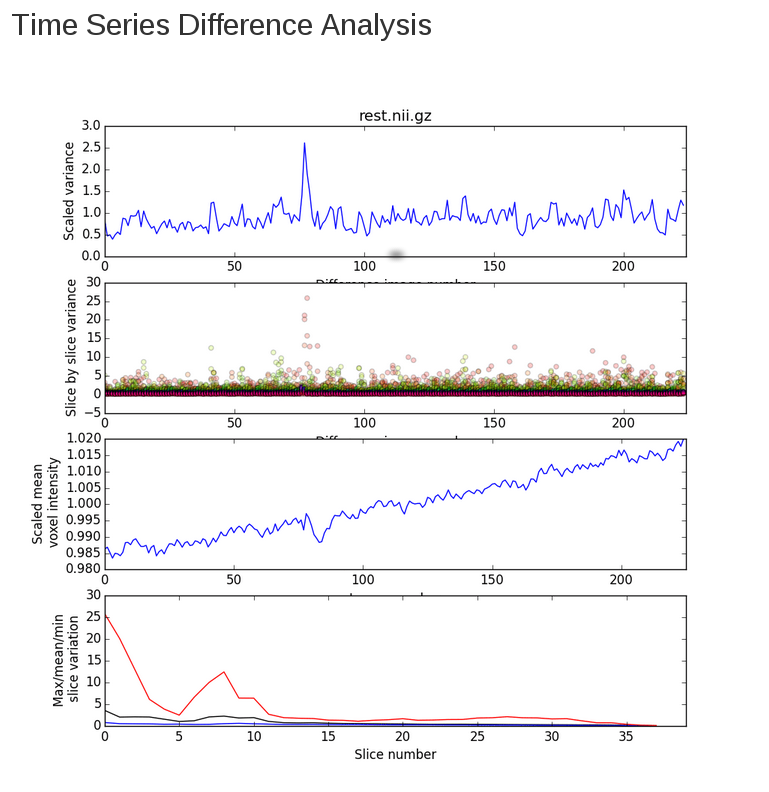
\includegraphics[scale=0.5]{images/QAtsdiffana.png}

\begin{lstlisting}
	MotionGraphs: QA/images/rest_MotionGraphRotations.gif 

	QA/images/rest_MotionGraphRotations.gif: rest_dir/rest_mc.nii.gz
		%*\lnote*$(PROJECT_HOME)/bin/R/MakingGraphs.Rscript  QA/images rest
\end{lstlisting}

\lnum{8}  \texttt{MakingGraphs.Rscript} is a R script that will generate 4 separate graphs for you: \\
	\tab 1. A motion rotations graph showing rotations along the x/y/z planes.\\
	\tab 2. A motion translations graph showing translations along the x/y/z planes.\\
	\tab 3. A framewise displacement (FD) graph to show displacement in mm across acquired volumes.\\
	\tab 4. A signal intensity (DVARS) graph to show signal intensity across acquired volumes.\\
	To understand the usage of an R script, it is usually necessary to look at the code itself. In this line, the R script called with the output directory \texttt{QA/images} as the first argument, followed by the prefix \texttt{rest} to be used for naming the output images.\\

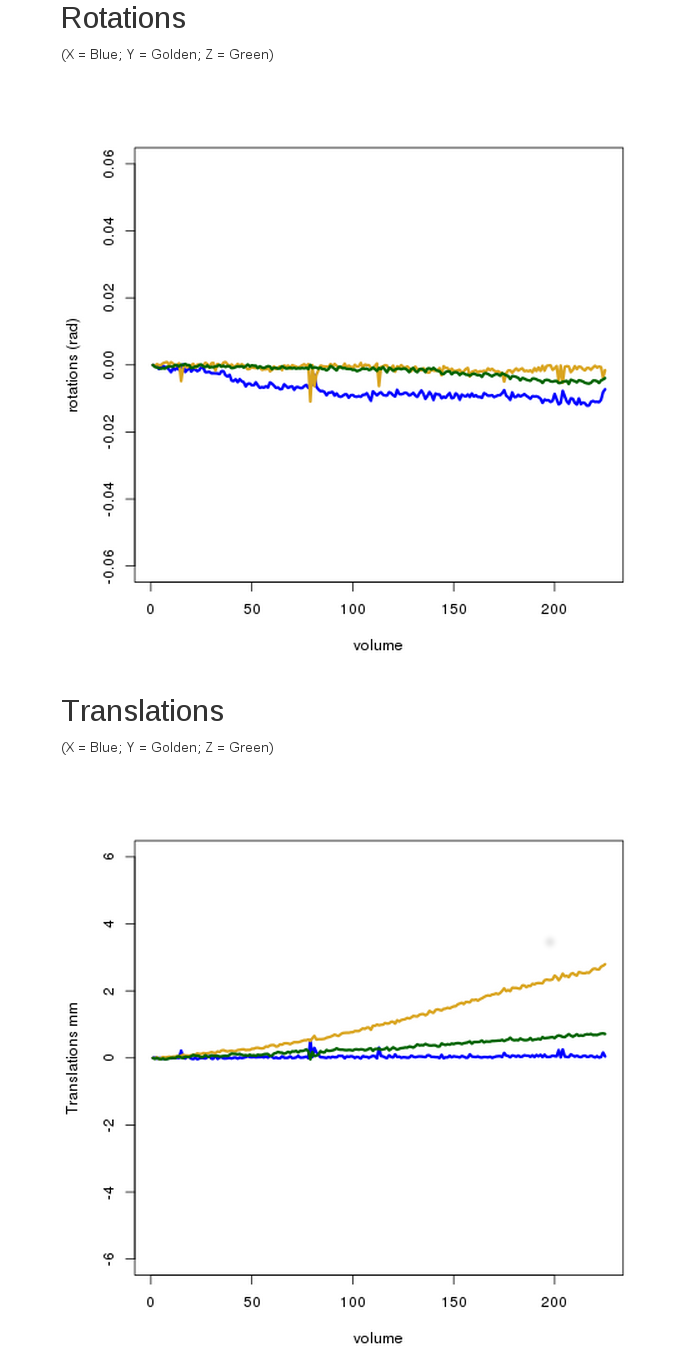
\includegraphics[scale=0.3]{images/QAmotion1.png}
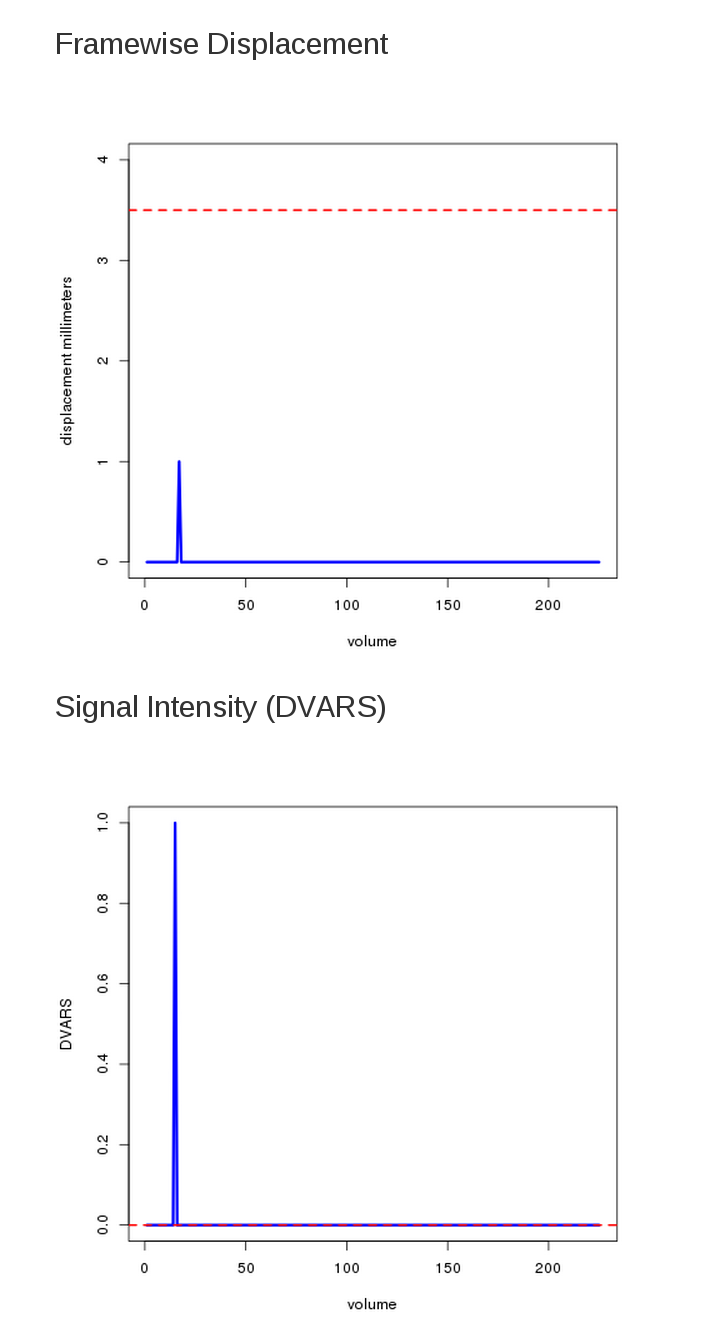
\includegraphics[scale=0.3]{images/QAmotion2.png}

\begin{lstlisting}
	SkullstripQA: QA/images/T1_skstrip.gif

	QA/images/T1_skstrip.gif: T1.nii.gz T1_skstrip_mask.nii.gz
		mkdir -p QA/images ;\
		%*\lnote*$(FSL_DIR)/bin/overlay 1 1 $< -a $(word 2,$^) 1 10 rendered_T1_brain.nii.gz ;\
		%*\lnote*$(PROJECT_HOME)/bin/slices rendered_T1_brain.nii.gz -o `dirname $@`/`basename $@ .gif`.png ;\
		%*\lnote*convert `dirname $@`/`basename $@ .gif`.png -resize 500 $@ ;\
		rm rendered_T1_brain.nii.gz ;\
		rm `dirname $@`/`basename $@ .gif`.png

\end{lstlisting}


To ensure that our skull-strip does not remove too much of the brain or too little of the skull, we can create an image to overlay the skull-stripped mask generated from \texttt{resting.mk} on top of the T1 brain. \\
\tab\lnum{9} FSL \texttt{overlay} is a tool that is used to overlay a 3D images over another. It is capable of overlaying a maximum of 2 images on top of a reference image. Type \texttt{overlay} into your command line to understand how it is used. In this line, we call \texttt{overlay}. The \texttt{1}s that are provided as arguments specify the color and output type of your overlay. The next argument is the background image, which in this case is the first dependency we have listed, i.e. \texttt{T1.nii.gz}. The \$\textasciicircum{} refers to this file. The final output image is called \texttt{rendered\_T1\_brain.nii.gz}. Again, to understand the flags, you must look at overlay's usage. \\
\lnum{10} FSL \texttt{slices} is a script that calls the FSL tool \texttt{slicer} to create an image consisting of 3 axial, 3 sagittal and 3 coronal slices. Here, we feed it the \texttt{rendered\_T1\_brain.nii.gz} file that we want FSL \texttt{slices} to use. The output will be a file called \texttt{QA/images/T1\_skstrip.png}. Instead of typing out the full name of the file, however, we simply provide the directory name and basename of our target and replace \texttt{.gif} with \texttt{.png}. \\
\lnum{11} Following this, we convert our PNG image into a GIF image, using ImageMagick's \texttt{convert} that performs the conversion and resizes the image.\footnote{This step was necessary in earlier versions of R Markdown that had trouble including PNG images, but may not be necessary for you.}\\

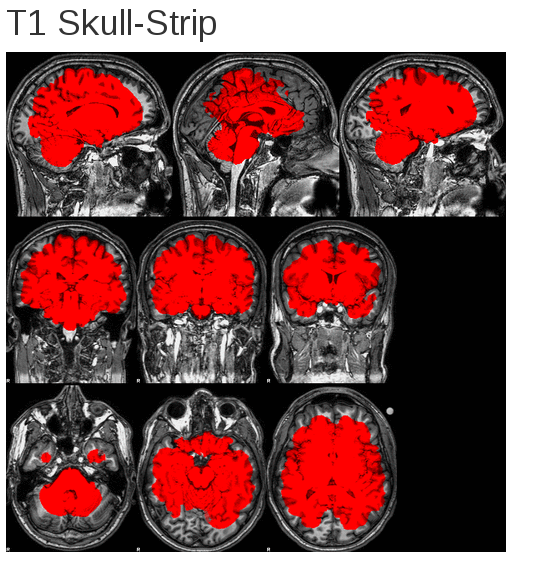
\includegraphics[scale=0.4]{images/QAskullstrip.png}

\begin{lstlisting}
	QAreport: QA/rest_Preprocessing.html 

	QA/rest_Preprocessing.html: $(PROJECT_HOME)/lib/Rmd/fMRI.Rmd TSNR MotionGraphs SkullstripQA
		%*\lnote*sed -e 's/SUBJECT/$(subject)/g' -e 's/TASK/rest/g' $(word 1,$^) > QA/rest_Preprocessing.Rmd ;\
		%*\lnote*R -e 'library("rmarkdown");rmarkdown::render("QA/rest_Preprocessing.Rmd")' ;\
		rm -f QA/rest_Preprocessing.Rmd QA/rest_Preprocessing.md
\end{lstlisting}


Finally, to generate our QA HTML report, we use R Markdown. We do this by writing a file called \texttt{fMRI.Rmd}, which is the first dependency listed here. The \texttt{fMRI.Rmd} file reads the QA images that were generated in the previous portions of this makefile to create a HTML page (see \nameref{sec:practicum4} for a brief explanation of what goes into a Rmd file and how to write one). \\
\lnum{12} In this line, we substitute pattern strings in the \texttt{fMRI.Rmd} file with variables that have been defined in the makefiles by using \texttt{sed}. \texttt{SUBJECT}, for instance, will be replaced with the \texttt{\$(subject)} variable defined in the main makefile \texttt{\$(PROJECT\_HOME)/test001/Makefile}. \texttt{TASK} will be replaced with \texttt{rest}, because we are only interested in looking at the QA report for resting-state functional scans for now. We can define another variable called \texttt{task} if we have several types of runs that we want to generate QA reports for (e.g., task runs or multiple resting state runs). Once the pattern strings have been substituted, the \texttt{fMRI.Rmd} file will be copied over to the \texttt{QA} directory and be renamed as \texttt{rest\_Preprocessing.Rmd}. \\
\lnum{13} This line tells R to load the `\texttt{rmarkdown}' library so that it can read the R Markdown file. R will then render \texttt{QA/rest\_Preprocessing.Rmd} to create your HTML report! \\

To view the full report, you can open the file \texttt{testsubject/test001/QA/rest_Preprocessing_example.html} in a browser.


\begin{lstlisting}
		clean_qa: 
		rm -rf QA
\end{lstlisting}

Finally, with other makefiles, we define a \texttt{clean} target specifically for QA. Because quality assurance is an intermediate step in the neuroimaging processing pipeline, we do not necessarily need to retain the QA images and reports once they have been checked.



